\section{Introduction}

In the previous chapters we discussed algorithms that operated on finite field elements as if they were made of individual bits (the binary coefficients). This is a sensible approach for building circuits, as the bits map naturally to simple signals, allowing the circuits to be constructed with basic logic gates. \\

However, during our research we also studied $GF(2^m)$ arithmetic for CPUs, where the individual bit approach is not efficient. In theory software could also operate on individual bits of each element, but this would require multiple instructions to process each bit, not to mention additional overhead on architectures incapable of addressing single bits. \\

On software implementations, the more sensible approach is to group the coefficients into CPU words. Given a polynomial $\sum_{i=0}^{m-1} d_i x^i$, we group the bits in words $D[0] \ldots D[t-1]$, each of length $W$, starting from $d_0 \ldots d_{W-1}$ (see Fig.~\ref{fig:elemento:field} for one possible case). However, this representation introduces a new layer of complexity to algorithms. Therefore, we decided to focus on the small but important area of polynomial reduction modulo a trinomial, a common operation in $\F_2[x]/(x^m+x^a+1)$. \\

This operation has some important practical applications. Using a trinomial as irreducible polynomial is preferred when available because it maximizes the number of zero coefficients in the the irreducible polynomial, enabling numerous simplifications. And the reduction operation is an important step for multiplications and exponentiations, making speedups desirable.\\

This chapter requires more notations and assumptions to represent CPU algorithms and words. We assume that one word has $W$ bits, where $W$ is a multiple of $8$. The bits of a word $A$ are numbered from $0$ to $W-1$, with the rightmost bit corresponding to the $x^0$ coefficient (LSB) of $A$ designated as bit $0$. The following standard notation is used to denote operations on words $A$ and $B$:\\

\begin{description}
\item[$A \BitXOR B$] bitwise exclusive or.
\item[$A \BitOr B$]  bitwise or. 
\item[$A \BitAnd B$]      bitwise $AND$.
\item[$A \ShiftLeft n$]      left shift of $A$ by $n$ positions, ($n<W$), with the bits from 0 to $n-1$ set to $0$. 
\item[$A\ShiftRight n$]     right shift of $A$ by $n$ positions, ($n<W$), with bits from $W-n$ to $W-1$ set to $0$. 
\end{description}

And the following variable naming:

\begin{description}
\item[$a, b, c, d$]  Polynomials in $\F_2[x]$, not necessarily an element of the field $\F_{2^m}$ (they may be an intermediate result before the final reduction).
\item[$A, B, C, D$]  Vector of bits corresponding to the polynomials $a, b, c, d$.
\end{description}

And because divisibility is paramount when grouping words into bits, outside algorithms we use the $x \mid y$ operator to indicate that "$x$ divides $y$", or $x \nmid y$ for "$x$ doesn't divide $y$".

In Section~\ref{operating-on-words} we give more details on the general differences of bit and word algorithms for this application. Section~\ref{delay-independence} shows an example of such difference. Section~\ref{bit-grouping} details the different cases of bit-grouping and how they lie across word boundaries. Section~\ref{helper-functions} contains helper functions that can be used to easily convert a bit-oriented algorithm to a word-oriented one.

\section{Operating on words}\label{operating-on-words}

Manipulation of individual bits is not efficient in most CPU architectures. In general, it is preferred to operate on words, with a size specific to the microprocessor architecture, such as $32$- or $64$-bit words. However, the reduction algorithms are strongly bit oriented, since the coefficients are not naturally grouped in words. The codification of these algorithms to word oriented programming languages usually adds some complexity in terms of bitwise shifts and masks, and doesn't enjoy the parallelism inherent in XOR circuits. Specific techniques that help us in this coding have been proposed in the literature\cite{Hilewitz2008}.  \\

In this scenario it's often desirable to have "interoperability", choosing a field size and a irreducible polynomial that leads to efficient operations in both hardware and software implementations. A straightforward approach to this problem is to develop a hardware implementation first, XOR'ing individual bits, and convert the algorithm to words. This can be thought of as parallelizing the operations, with SHIFTs and AND/OR masks for alignment. This is the approach used in this work. \\

The difficulty of the conversion process greatly varies depending on the access pattern of the algorithm and alignment of words. If all coefficients inside a range are XOR'ed once in a linear fashion, the XOR distance a multiple of the word size, and the start and end range lie in word boundaries, the converted algorithm gains a full speedup of up to \texttt{WORD\_SIZE} times {[}$C_{word} = \ceil*{\frac{C_{bit}}{W}}${]}. \\

The word-oriented algorithm can be helped by choosing specific field sizes and irreducible polynomials that introduce operations aligning at word boundaries, to avoid these bitwise shifts and masks, or that map well to architecture-specific operations. In our algorithms we try to make use of alignment opportunities when they appear, but do not depend on them or any specific architecture. \\

\section{Delay independence}\label{delay-independence}

Performing binary polynomial reduction in a CPU has a few differences from implementing a hardware circuit. For example, circuits often avoid irreducible polynomials with the second largest exponent $a > \ceil{m/2}$. As seen before with pentanomials, this characteristic leads to higher delays in most circuit-based reduction algorithms. This is caused by the inter-dependency of the calculations, limiting the natural parallelism of circuits and thus increases the total delay. \\

This property does not affect software implementations. To illustrate this, we take two algorithms that perform modular reduction for the NIST irreducible trinomials $x^{233} + x^{74} + 1$ and $x^{409} + x^{87} + 1$, as implemented in the literature~\cite[p. 55]{hankerson2006guide}. \\

The original algorithms are Algorithm~\ref{alg:233_74_nist} (which reduces a polynomial modulo $x^{233} + x^{74} + 1$) and Algorithm~\ref{alg:409_87_nist} (modulo $x^{409} + x^{87} + 1$). These algorithms are similar to our Algorithm~\ref{alg:reduce}, but optimized for word processing. To process multiple bits at once, entire words are XOR'ed together. And to ensure the bits line up, left and right shifts are used. The temporary variable $T$ is used to avoid recomputing the same array indexing twice, while the final mask in each algorithm is to "truncate" the reduction result. \\

Based on these algorithms, we manually adapted each to perform a reduction modulo its reciprocal irreducible trinomial. The reciprocal of a trinomial $x^m + x^a +1$ is the trinomial $x^m + x^{a-m} + 1$, and they hold the interesting property that if the first one is irreducible, then so is the second. In this case, this property ensures that the adapted algorithm is still reducing modulo an irreducible trinomial. \\

The adapted versions are Algorithm~\ref{alg:233_159} (which reduces modulo $x^{233} + x^{159} + 1$ instead of $x^{233} + x^{74} + 1$), and Algorithm~\ref{alg:409_322} (modulo $x^{409} + x^{322} + 1$ instead of $x^{409} + x^{87} + 1$). Note that the number, type and order of the instructions is exactly the same. The only changes required were on the constants, more specifically the array indexing and shifting constants. Therefore the adapted versions have the exact same performance characteristics. \\

This is important because the bit-level algorithms would have different delays, as the delay depends on the distance $m-a$. This means there are some non-obvious differences between bit- and word-level algorithms, and that some of these differences actually lead to simpler properties, like the $a$-independent delay seen here. \\

\begin{algorithm}
  \caption{Hankerson's algorithm for reduction modulus $x^{233} + x^{74} + 1$, a standardized NIST polynomial.}
  \label{alg:233_74_nist}
\begin{algorithmic}[1]
  \REQUIRE $C[2m-2,0]$
  \ENSURE $C[m-1,0]$
  \FOR{$i \gets 15$ \textbf{downto} $8$}
    \STATE $T \gets C[i]$
    \STATE $C[i-8] \gets C[i-8] \oplus T << 23$
    \STATE $C[i-7] \gets C[i-7] \oplus T >> 9$
    \STATE $C[i-5] \gets C[i-5] \oplus T << 1$
    \STATE $C[i-4] \gets C[i-4] \oplus T >> 31$
  \ENDFOR
  \STATE $T \gets C[7] >> 9$
  \STATE $C[0] \gets C[0] \oplus T$
  \STATE $C[2] \gets C[2] \oplus T << 10$
  \STATE $C[3] \gets C[3] \oplus T >> 22$
  \STATE $C[7] \gets C[7] \& \texttt{0x1FF}$
  \RETURN $C$
\end{algorithmic}
\end{algorithm}

 \begin{algorithm}
  \caption{Algorithm for reduction modulus $x^{233} + x^{159} + 1$, $(233, 74)$'s reciprocal.}
  \label{alg:233_159}
 \begin{algorithmic}[1]
  \REQUIRE $C[2m-2,0]$
  \ENSURE $C[m-1,0]$
  \FOR{$i \gets 14$ \textbf{downto} $8$}
    \STATE $T \gets C[i]$
    \STATE $C[i-8] \gets C[i-8] \oplus T << 23$
    \STATE $C[i-7] \gets C[i-7] \oplus T >> 9$
    \STATE $C[i-3] \gets C[i-3] \oplus T << 22$
    \STATE $C[i-2] \gets C[i-2] \oplus T >> 10$
  \ENDFOR
  \STATE $T \gets C[7] >> 9$
  \STATE $C[0] \gets C[0] \oplus T$
  \STATE $C[2] \gets C[2] \oplus T << 31$
  \STATE $C[3] \gets C[3] \oplus T >> 1$
  \STATE $C[7] \gets C[7] \& \texttt{0x1FF}$
  \RETURN $C$
\end{algorithmic}
\end{algorithm}

\begin{algorithm}
  \caption{Hankerson's algorithm for reduction modulus $x^{409} + x^{87} + 1$, a standardized NIST polynomial.}
  \label{alg:409_87_nist}
\begin{algorithmic}[1]
  \REQUIRE $C[2m-2,0]$
  \ENSURE $C[m-1,0]$
  \FOR{$i \gets 25$ \textbf{downto} $13$}
    \STATE $T \gets C[i]$
    \STATE $C[i-13] \gets C[i-13] \oplus T << 7$
    \STATE $C[i-12] \gets C[i-12] \oplus T >> 25$
    \STATE $C[i-11] \gets C[i-11] \oplus T << 30$
    \STATE $C[i-10] \gets C[i-10] \oplus T >> 2$
  \ENDFOR
  \STATE $T \gets C[12] >> 25$
  \STATE $C[0] \gets C[0] \oplus T$
  \STATE $C[2] \gets C[2] \oplus T << 23$
  \STATE $C[12] \gets C[12] \& \texttt{0x1FFFFFF}$
  \RETURN $C$
\end{algorithmic}
\end{algorithm}


\begin{algorithm}
  \caption{Algorithm for reduction modulus $x^{409} + x^{322} + 1$, $(409, 87)$'s reciprocal.}
  \label{alg:409_322}
\begin{algorithmic}[1]
  \REQUIRE $C[2m-2,0]$
  \ENSURE $C[m-1,0]$
  \FOR{$i \gets 25$ \textbf{downto} $13$}
    \STATE $T \gets C[i]$
    \STATE $C[i-13] \gets C[i-13] \oplus T << 7$
    \STATE $C[i-12] \gets C[i-12] \oplus T >> 25$
    \STATE $C[i-3] \gets C[i-3] \oplus T << 9$
    \STATE $C[i-2] \gets C[i-2] \oplus T >> 23$
  \ENDFOR
  \STATE $T \gets C[12] >> 25$
  \STATE $C[0] \gets C[0] \oplus T$
  \STATE $C[10] \gets C[10] \oplus T << 2$
  \STATE $C[12] \gets C[12] \& \texttt{0x1FFFFFF}$
  \RETURN $C$
\end{algorithmic}
\end{algorithm}

\section{Bit grouping}\label{bit-grouping}

In this chapter's introduction it was mentioned that word-level algorithms group the bits into words, and Figure~\ref{fig:elemento:field} was given as an example of such packing. However this is not the only arrangement that can happen. Depending on the relationship between the word size $W$ and the irreducible polynomial degree $m$, the last bits may be packed in different ways. \\

Figure~\ref{fig:elemento:field} shows the representation of a element $d \in \ftwom$ as an array $D$ of $t$ words of $W$ bits, where $t = \left \lceil \frac{m}{W} \right \rceil$. The $s = tW-m$ highest order bits of $D[t-1]$ are not unused.
\begin{figure}[htb]
  \centering
  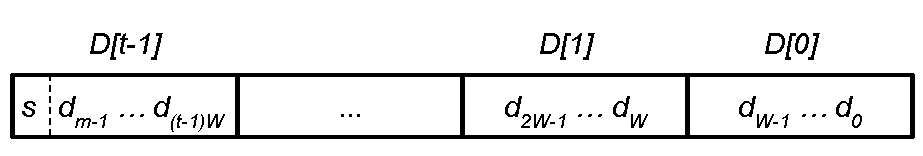
\includegraphics[width = .55\columnwidth]{figures/element-word.pdf}
\caption{Representation of $d \in \ftwom$ as an array $D$ of $W$ bit words. The $s = tW-m$ highest order bits of $D[t-1]$ are not unused.}
\label{fig:elemento:field}
\end{figure}
\\

For the case where $(m-1) \mod{W} > \frac{W}{2}$, the Figure~\ref{fig:elemento:field:mult} shows the representation of an element $d = ab$, $a,b \in \ftwom$ as an array $D$ of $W$-bit words. The $s = 2(tW-m)+1$ highest order bits of $D[2t-1]$ are not unused. \\

\begin{figure}
  \centering
  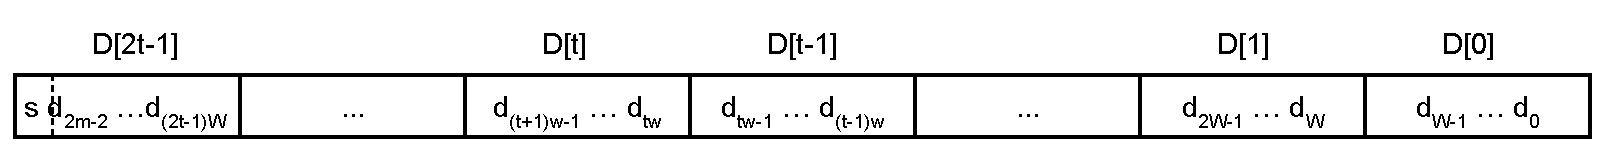
\includegraphics[width = .9\columnwidth]{figures/two-word-element-1.pdf}
\caption{Representation of $d = ab$, $a,b \in \ftwom$ as an array $D$ of $W$-bit words. The $s = 2(tW-m)+1$ highest order bits of $D[2t-1]$ are not unused.}
\label{fig:elemento:field:mult}
\end{figure}


When $(m-1) \mod{W} \leq \frac{W}{2}$, $D[2t-1]$ is not needed.  Figure~\ref{fig:elemento:field:mult2} shows the representation of a element $d = ab$, $a,b \in \ftwom$ as an array $D$ of $W$-bit words. The $s = 2(tW-m)+1$ highest order bits of $D[2t-2]$ and $D[2t-1]$ are not unused. \\

\begin{figure}
  \centering
  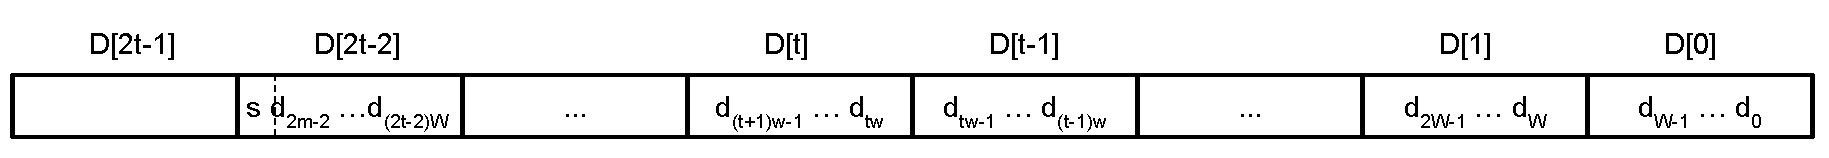
\includegraphics[width = \columnwidth]{figures/two-word-element-2.pdf}
\caption{Representation of $d = ab$, $a,b \in \ftwom$ as an array $D$ of $W$-bit words. The $s = 2(tW-m)+1$ highest order bits of $D[2t-2]$ and $D[2t-1]$ are not unused.}
\label{fig:elemento:field:mult2}
\end{figure}

In these cases a whole word is wasted, but length calculations become simpler: to get the length (in words) of a product of two elements, just add their lengths (in words). \\


\section{Helper functions for conversion} \label{helper-functions}

The word-oriented versions of bit-level reduction algorithms can be created by noticing the bit access pattern. These patterns are fairly regular, XOR'in the bit $c_i$ with $c_j$, followed by $c_{i+1}$ with $c_{j+1}$, etc. The algorithm can be split into these regular patterns, and the patterns can be thought of as XOR'ing two ranges. \\

Each of these patterns perform a XOR operation between all bits in a certain range and counterparts a fixed distance away. This access pattern allows word-level parallelism. To exemplify the process of converting a bit-level algorithm to word-level, we take the reduction algorithm Algorithm~\ref{alg:reduce} shown in Chapter~\ref{chapters/reduction_squaring_2}, and for simplicity we adapt it to the specific case of reduction modulo a trinomial $x^m + x^a + 1$ and $a=\frac{m}{2}$ (also called "equally spaced trinomial"), creating Algorithm~\ref{alg:reduce_trinomial}.

\begin{algorithm}
\caption{Modular reduction for equally-spaced irreducible trinomials in $GF(2^m)$}
\label{alg:reduce_trinomial}
\begin{algorithmic}[1]
\REQUIRE $C = [c_0, c_1, c_2, ..., c_d]$, $d \geq m$, $f(x) = x^m + x^{m/2} + 1$
\ENSURE $C \mod f$
  \FOR{$i \leftarrow 0$ \textbf{to} $m-2$}
    \STATE $C[i+a] \leftarrow C[i+a] \oplus C[i+m]$
  \ENDFOR
  \FOR{$i \leftarrow a - 1$ \textbf{to} $0$}
    \STATE $C[i] \leftarrow C[i] \oplus C[i+m]$
  \ENDFOR
\RETURN $C[0],~C[1],~C[2],~\ldots,~C[m-1]$
\end{algorithmic}
\end{algorithm}

There are four issues that need to be paid attention to:

\textbf{Misaligned start:}
The ranges starts may not align with the word length ($W \nmid 2m-2$). To avoid overwriting the upper bits of this incomplete word we must clear them from the \texttt{src} word. \\

\textbf{Misaligned ends:}
The fix is identical to the misaligned start, where we clear the extra bits from the incoming word. \\

\textbf{Misaligned source:}
The source/incoming word may not be aligned to word boundaries either. In this case we need to pull bits from the next word too, shifting both of them for correct placement. Unfortunately this issue affects the start and ends word too, further complicating their treatment. \\

\textbf{Too small distances:}
Finally, if the distance between the XOR'ed words ($m-a$, $m$, respectively) is smaller than $W/2$, the same bit will be written and read in the same word-step. This is not possible with a single operation, and requires handling each word in multiple parts. This is suboptimal and should be avoided by better choices of $m$, $a$ and $W$. \\

Other bit-level operations are emulated with word masks and shifts. \\

To help transforming an algorithm in its word-level version we introduce the following helper functions. Notice the function calls can be inlined and all conditionals are possible to be analyzed statically, therefore the final algorithm should contain no conditionals if optimized properly. \\

Algorithm~\ref{alg:xor_bit} performs a XOR operation of a single bit. Algorithm~\ref{alg:xor_word} XOR's a full word with another word some distance away, with the source possibly misaligned. Algorithm~\ref{alg:xor_partial_word} is able to XOR only a range of bits inside a word, instead of the full word. Finally, Algorithm~\ref{alg:xor_range} uses the previous two algorithms two XOR an arbitrary range. \\

\begin{algorithm}
\caption{\texttt{XOR\_BIT}: Single bit XOR inside word}
\label{alg:xor_bit}
\begin{algorithmic}[1]
  \REQUIRE $dst$, $src$, $W$, $C[]$
  \STATE $mask \gets 1 << (src \mod W)$
  \STATE $C[dst / W] \gets C[dst / W] \oplus (C[src / W] \land mask) << (dst \mod W - src \mod W)$
\end{algorithmic}
\end{algorithm}

\begin{algorithm}
\caption{\texttt{XOR\_WORD}: Whole word XOR with possibly misaligned source}
\label{alg:xor_word}
\begin{algorithmic}[1]
  \REQUIRE $dst$, $src$, $W$, $C[]$
  \STATE $left \gets C[src / W] >> (src \mod W)$
  \STATE $right \gets C[src / W + 1] << (W - src \mod W)$
  \STATE $C[dst / W] \gets C[dst / W] \oplus (left \lor right)$
\end{algorithmic}
\end{algorithm}

\begin{algorithm}
\begin{algorithmic}[1]
  \REQUIRE $dst$, $src$, $n\_bits$, $W$, $C[]$
  \STATE $shift \gets src \mod W$
  \STATE $left\_n\_bits \gets \min(n\_bits, W - shift)$
  \STATE $leftmask \gets ((1 << left\_n\_bits) - 1) << shift$
  \STATE $left \gets (C[src / W] \land leftmask) >> shift$
  \STATE $right\_n\_bits \gets n\_bits - left\_n\_bits$
  \IF{$right\_n\_bits > 0$}
    \STATE $rightmask \gets (1 << right\_n\_bits) - 1$
    \STATE $right \gets (C[src/W+1] \land rightmask) << left\_n\_bits$
  \ELSE
    \STATE $right \gets 0$
  \ENDIF
  \STATE $C[dst/W] = C[dst/W] \oplus ((left | right) << (dst \ W))$
  \caption{\texttt{XOR\_PARTIAL\_WORD}: XOR a range of bits inside a word, with possibly misaligned source}
  \label{alg:xor_partial_word}
\end{algorithmic}
\end{algorithm}

\begin{algorithm}
\begin{algorithmic}[1]
  \REQUIRE $start\_dst$, $end\_dst$, $distance$, $W$, $C[]$
  \IF{$end\_dst/W = start\_dst/W$}
    \STATE \texttt{XOR\_PARTIAL\_WORD}($start\_dst$, $start\_dst + distance$, $end\_dst - start\_dst$, $W$, $C$)
  \ELSE
    \IF{$start\_dst \ W \neq 0$}
      \STATE $remaining = W - (start\_dst \ W)$
      \STATE \texttt{XOR\_PARTIAL\_WORD}($start\_dst$, $start\_dst + distance$, $remaining$, $W$, $C$)
      \STATE $start\_dst \gets start\_dst + remaining$
    \ENDIF
    
    \STATE $rounded\_end \gets (end\_dst / W) * W$
    \STATE $dst \gets start\_dst$
    \WHILE{$dst < rounded\_end$}
      \STATE \texttt{XOR\_WORD}($dst$, $dst + distance$, $W$, $C$)
      \STATE $dst \gets dst + W$
    \ENDWHILE
    
    \IF{$end\_dst \ W \neq 0$}
      \STATE \texttt{XOR\_PARTIAL\_WORD}($rounded\_end$, $rounded\_end + distance$, $end\_dst \ W$, $W$, $C$)
    \ENDIF
  \ENDIF
  \label{alg:xor_range}
  \caption{\texttt{XOR\_RANGE}: XOR a range of bits (across many words) with an equivalent range a certain distance away}
\end{algorithmic}
\end{algorithm}

Now we are ready to adapt our example bit-level reduction algorithm, Algorithm~\ref{alg:reduce_trinomial}. The trivially transformed version is seen in Algorithm~\ref{alg:equallyspaced:word:operation}, where the XOR inside the "for" loops were simply replaced with \texttt{XOR\_RANGE} calls. \\

\begin{algorithm}
\begin{algorithmic}[1]
  \REQUIRE $m$, $a$, $W$, $C\left[0,\ceil*{\frac{2m-2}{W}}\right]$
  \ENSURE $C[0,m-1]$
  \STATE \texttt{XOR\_RANGE}($a$, $a+m$, $m$, $W$, $C$)
  \STATE \texttt{XOR\_RANGE}($0$, $a-1$, $m$, $W$, $C$)
  \RETURN $C$
  \caption{Simple word-parallel reduction algorithm for $x^m + x^a +1$, $a = \frac{m}{2}$}
  \label{alg:equallyspaced:word:operation}
\end{algorithmic}
\end{algorithm}

As an example of the final result to be expected, we adapted our general reduction algorithm to perform reductions modulo the NIST trinomial $x^{233} + x^{74} + 1$ and 32-bit words. Then we inlined all functions and removed the conditional branches through static analysis. This effort resulted in algorithm \ref{alg:233-32:word:operation}.

\begin{algorithm}
\begin{algorithmic}[1]
  \REQUIRE $C\left[0,\ceil*{\frac{2m-2}{W}}\right]$
  \ENSURE $C[0,m-1]$
  \STATE $C[2] \gets C[2] \oplus ((C[7] \land \texttt{0x7ffffe00}) << 1)$
  \STATE $C[3] \gets C[3] \oplus ((C[7] >> 31) \lor (C[8] << 1))$
  \STATE $C[4] \gets C[4] \oplus ((C[8] >> 31) \lor (C[9] << 1))$
  \STATE $C[5] \gets C[5] \oplus ((C[9] >> 31) \lor (C[10] << 1))$
  \STATE $C[6] \gets C[6] \oplus ((C[10] >> 31) \lor (C[11] << 1))$
  \STATE $C[7] \gets C[7] \oplus ((C[11] >> 31) \lor (C[12] << 1))$
  \STATE $C[8] \gets C[8] \oplus ((C[12] >> 31) \lor (C[13] << 1))$
  \STATE $C[9] \gets C[9] \oplus ((C[13] >> 31) \lor ((C[14] \land \texttt{0x1ffff}) >> 1))$
  \STATE $C[2] \gets C[2] \oplus ((C[12] \land \texttt{0x3fffff00}) << 2)$
  \STATE $C[3] \gets C[3] \oplus ((C[12] >> 30) \lor (C[13] << 2))$
  \STATE $C[4] \gets C[4] \oplus ((C[13] >> 30) \lor ((C[14] \land \texttt{0x1ffff}) >> 2))$
  \STATE $C[0] \gets C[0] \oplus ((C[7] >> 9) \lor (C[8] << 23))$
  \STATE $C[1] \gets C[1] \oplus ((C[8] >> 9) \lor (C[9] << 23))$
  \STATE $C[2] \gets C[2] \oplus ((C[9] >> 9) \lor (C[10] << 23))$
  \STATE $C[3] \gets C[3] \oplus ((C[10] >> 9) \lor (C[11] << 23))$
  \STATE $C[4] \gets C[4] \oplus ((C[11] >> 9) \lor (C[12] << 23))$
  \STATE $C[5] \gets C[5] \oplus ((C[12] >> 9) \lor (C[13] << 23))$
  \STATE $C[6] \gets C[6] \oplus ((C[13] >> 9) \lor (C[14] << 23))$
  \STATE $C[7] \gets C[7] \oplus ((C[14] \land \texttt{0x3fe00}) >> 9)$
  \RETURN $C$
  \caption{Reduction algorithm for $x^{233} + x^{74} + 1$ with 32-bit words}
  \label{alg:233-32:word:operation}
\end{algorithmic}
\end{algorithm}

Since this algorithm performs the same function as Algorithm~\ref{alg:233_74_nist} from literature, we can directly compare the total number of operations in them, seen in Table~\ref{table:comparison:nist}. Our implementation is less efficient, but still achieved a good result for an approach that is little more than a translation. \\

\begin{table}
\centering
\caption{Comparison of number of operations of our adapted algorithm and Algorithm~\ref{alg:233_74_nist}~\cite[p. 55]{hankerson2006guide}.}
{\begin{tabular}{l l l l l l} \label{table:comparison:nist}
Algorithm & \# XORs & \# ORs & \# SHIFTs & \# ANDs & Total \\ \hline
Ours & 16 & 16 & 35 & 5 & 75 \\ \hline
Algorithm~\ref{alg:233_74_nist} & 35 & 0 & 35 & 1 & 71
\end{tabular}}{}
\end{table}

With further improvements to the helper functions, and possibly manual tweaking of output, it may be possible to improve on the state of the art with this approach. Furthermore, this open the possibility of automatic code generation for little researched binary finite fields, since there's less work required to implement efficient arithmetic in such fields.